\section{Face detection}
We used Haar Cascade classifiers \cite{haar_cascade} proposed by Paul Viola and Michael Jones in order to achieve this task. First, we use our trained model to detect a person, then the ROI of that person is passed to the face detector. The face detector performs the algorithm to check if a person is facing a painting, based on these following scenarios:
\begin{enumerate}[label=\alph*)]
    \item Face found
    \begin{enumerate}[label=(\roman*)]
        \item \label{Eyes found} Eyes found (at least one)
        \item \label{Eyes not found} Eyes not found
    \end{enumerate}
    \item \label{Face not found} Face not found
\end{enumerate}

\begin{figure}[h!]
    \centering
    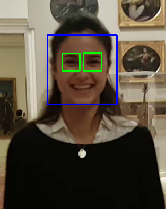
\includegraphics[width=0.2\textwidth]{pictures/face_detection/face_det2}
    \caption{the case in which the face detector correctly found a face from the person ROI}
    \label{fig:Eyes}
\end{figure}

In case \ref*{Eyes found}, if the face is found with its eyes, we assume that the person is facing the camera therefore he is not facing a painting, like in fig. \ref{fig:Eyes}.
\begin{figure}[h!]
    \centering
    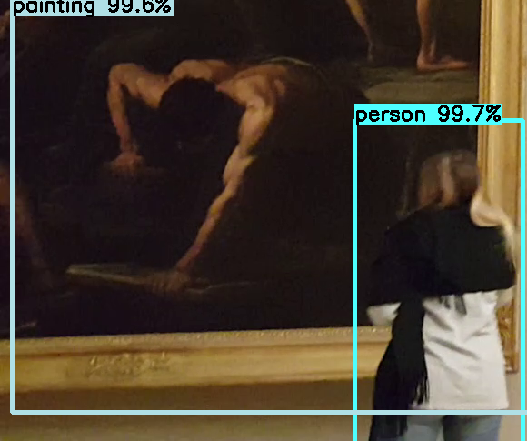
\includegraphics[width=0.3\textwidth]{pictures/face_detection/face_det1}
    \caption{the case where the face detector can't find the face}
    \label{fig:No_eyes}
\end{figure}
In case \ref*{Eyes not found}, if the face is found but the eyes are not detected, we assume that the person is facing a painting, this case is a particular scenario where the person could be in profile. The case \ref*{Face not found} has the same assumptions of the case \ref*{Eyes not found} because if the face is not detected, this could mean that the person is turning his back to the camera and, therefore, is possibly facing a painting, like in fig \ref{fig:No_eyes}. In these last scenarios, we take into account the paintings ROIs and we check if the person ROI overlaps a painting ROI, in this case the person is in front of a painting.

\subsection{Evaluation}
The assumptions we've made, have allowed us to model most of the possible cases, but since the videos where there is a clearly visible person are only few, the test evaluation may not represent the real accuracy of our approach. As a result, the test has been done using 2 frames per second for each videos where there is at least one person for more than 3 seconds, with a total of 8 videos. 466 are the total frames used and only 121 are the optimal candidates for the test, where a person is clearly visible, and was not too far from the camera. Since the face detector takes in input the person and paintings ROIs, our test is also affected by the quality of our trained model, therefore, not detecting some of the people and paintings, led us to discard another 42 frames.

After all of these reductions, we analyzed a total of 84 frames with 94 people inside it. The evaluation results are shown in table \ref{tab:face_detection_eval} and gave us an accuracy of: \[Accuracy = \frac{14+57}{94} \approx 0.85\]

\begin{table}[]
    \centering
    \begin{tabular}{cccc}
        & & \multicolumn{2}{c}{\textit{Facing painting}}                                                      \\ \cline{3-4}
        & \multicolumn{1}{c|}{}              & \multicolumn{1}{c|}{\textbf{True}}              & \multicolumn{1}{c|}{\textbf{False}}             \\ \cline{2-4}
        \multicolumn{1}{c|}{} & \multicolumn{1}{c|}{\textbf{True}} & \multicolumn{1}{c|}{14} & \multicolumn{1}{c|}{10} \\ \cline{2-4}
        \multicolumn{1}{c|}{\multirow{-2}{*}{\textit{\begin{tabular}[c]{@{}c@{}}
                                                         Face detector\\ answer
        \end{tabular}}}} &
        \multicolumn{1}{c|}{\textbf{False}} &
        \multicolumn{1}{c|}{13} &
        \multicolumn{1}{c|}{57} \\ \cline{2-4}
    \end{tabular}%
    \caption{Face detection results}
    \label{tab:face_detection_eval}
\end{table}